
\section{Study of Parallel Workload \Rmnum{2 }}
%\section{``Bully" become ``bullied"}
\label{sec:workload-2}

In this section, we will verify the observations made in the previous section 
when Workload~\Rmnum{1} is running on the dragonfly network under different placement and routing configurations. 
We conduct the same sets of experiments with Workload~\Rmnum{2}, which consists of sAMG, MultiGrid and CrystalRouter. 
By replacing AMG with sAMG, we turn the ``bully" into the ``bullied".


\subsection{Network Performance Analysis}
\label{sec: workload-2 network analysis}


Due to the replacement of AMG by sAMg, 
the volume of data transfer in Workload~\Rmnum{2} is much higher than Workload~\Rmnum{1}, 
thus the aggregate traffic on terminal links, local and global channels is greatly increased, 
as shown in Figure~\ref{fig:synwkld-network-traffic-stime}. 
The similar pattern in Figure~\ref{fig:wkld-network-traffic-stime} can be observed from Figure~\ref{fig:synwkld-network-traffic-stime}.
Contiguous placement coupled with minimal routing(CM) results in congestion on some routers along certain shortest paths from the source to the destination. 
Those congested routers are over-loaded with high volume of traffic going through their local and global channels, 
shown as the blue dashed line in Figure~\ref{fig:synwkld-global-channel-traffic} and~\ref{fig:synwkld-local-channel-traffic}. 
In the meanwhile, the corresponding saturated time of their local and global channels are also the highest compared with other configurations, 
shown as the blue dashed line in Figure~\ref{fig:synwkld-global-channel-stime} and Figure~\ref{fig:synwkld-local-channel-stime}. 

When contiguous placement coupled with (progressive) adaptive routing is in use, the high volume of traffic are redirected by taking the intermediate routers in other groups to void congestion. Therefore, the traffic on the global channels can be uniformly distributed over the network and the corresponding saturated time are greatly reduced, illustrated by the red and green dashed lines. However, (progressive) adaptive routing can not effectively balance the traffic load for local channels. As shown by the red and green dashed lines in Figure~\ref{fig:synwkld-local-channel-traffic}, some routers still have high volume of traffic on their local channels. 


Random placement policy performs comparably with three different routing policies.
By uniformly distributing MPI ranks over the network, 
random placement can balance the traffic load over the network,
illustrated by the solid lines in Figure~\ref{fig:synwkld-global-channel-traffic} and~\ref{fig:synwkld-local-channel-traffic}. 
Progressive adaptive and adaptive routing generate more traffic than minimal routing
as the packets take non-shortest paths via intermediate routers to avoid congestions, 
thus the blue solid line(RM) is lower than the red and green solid line (RA, RPA).



\begin{figure*}[t]
    \centering
    \begin{subfigure}[t]{0.32\textwidth}
        \centering
        \includegraphics[height=1.8 in]{syn-wkld/gc-traffic}
        \caption{Global Channel Traffic}
        \label{fig:synwkld-global-channel-traffic}
    \end{subfigure}\hfill
    \hspace{1em}%
    \begin{subfigure}[t]{0.32\textwidth}
        \centering
        \includegraphics[height=1.8 in]{syn-wkld/lc-traffic}
        \caption{Local Channel Traffic}
        \label{fig:synwkld-local-channel-traffic}
    \end{subfigure}\hfill
    \hspace{1em}%
    \begin{subfigure}[t]{0.32\textwidth}
        \centering
        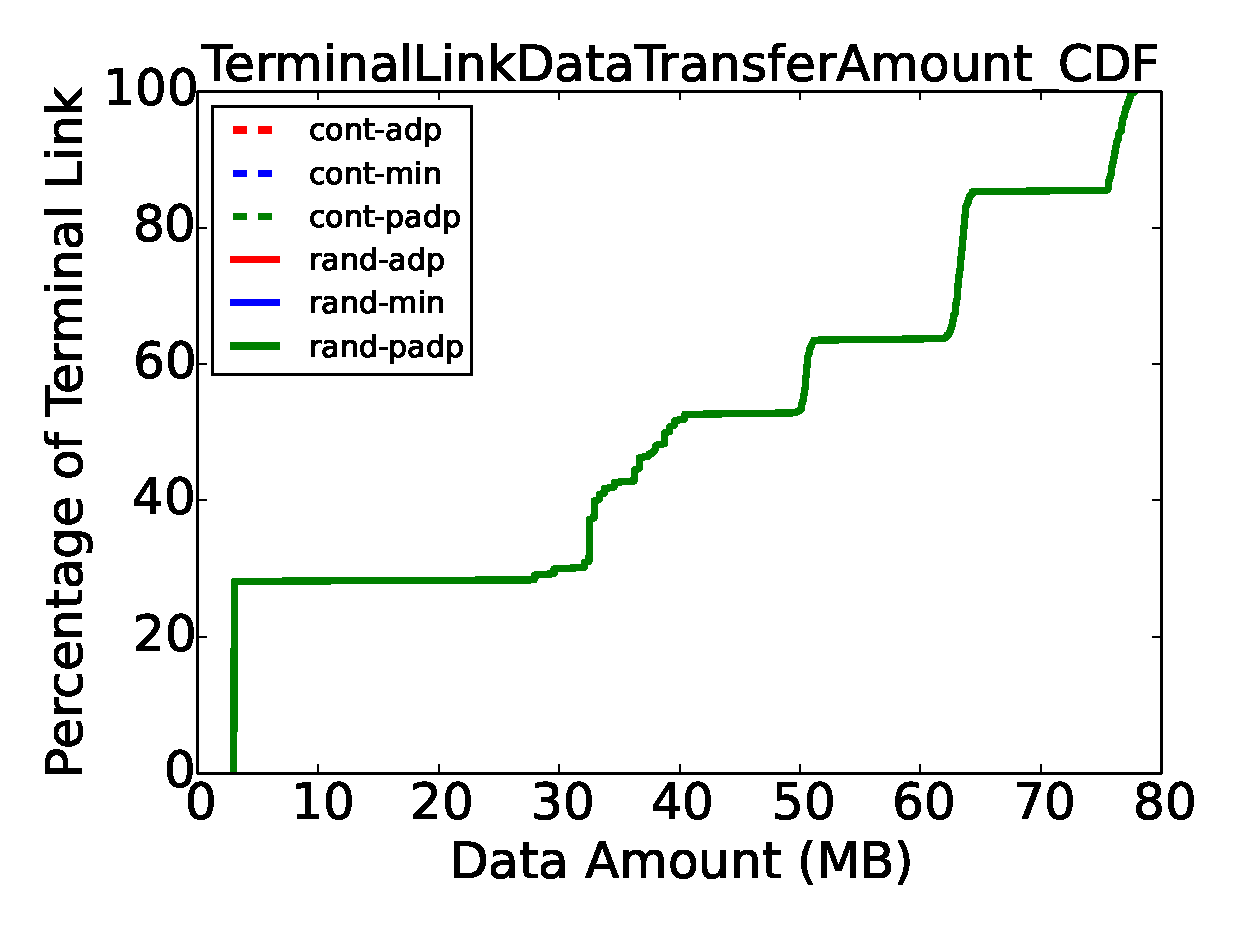
\includegraphics[height=1.8 in]{syn-wkld/tl-traffic}
        \caption{Terminal Link Traffic}
        \label{fig:synwkld-terminal-link-traffic}
    \end{subfigure}\\

    \begin{subfigure}[t]{0.32\textwidth}
        \centering
        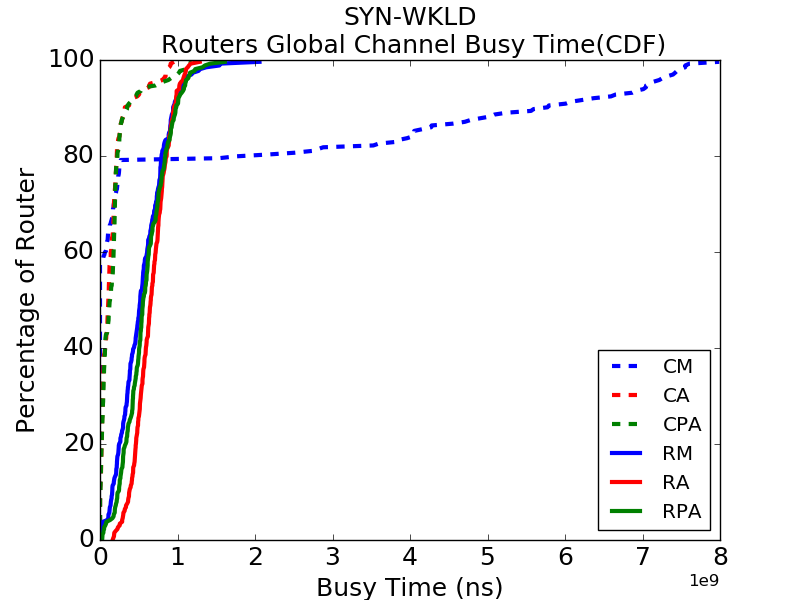
\includegraphics[height=1.8 in]{syn-wkld/gc-btime}
        \caption{Global Channel Saturated Time}
        \label{fig:synwkld-global-channel-stime}
    \end{subfigure}\hfill
     \hspace{1em}%
    \begin{subfigure}[t]{0.32\textwidth}
        \centering
        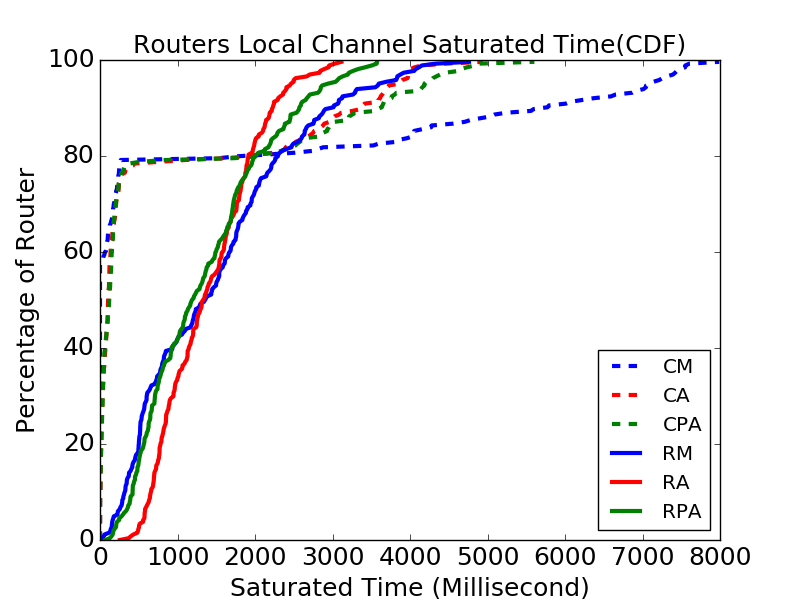
\includegraphics[height=1.8 in]{syn-wkld/lc-btime}
        \caption{Local Channel Saturated Time}
        \label{fig:synwkld-local-channel-stime}
    \end{subfigure}\hfill
    \hspace{1em}%
    \begin{subfigure}[t]{0.32\textwidth}
        \centering
        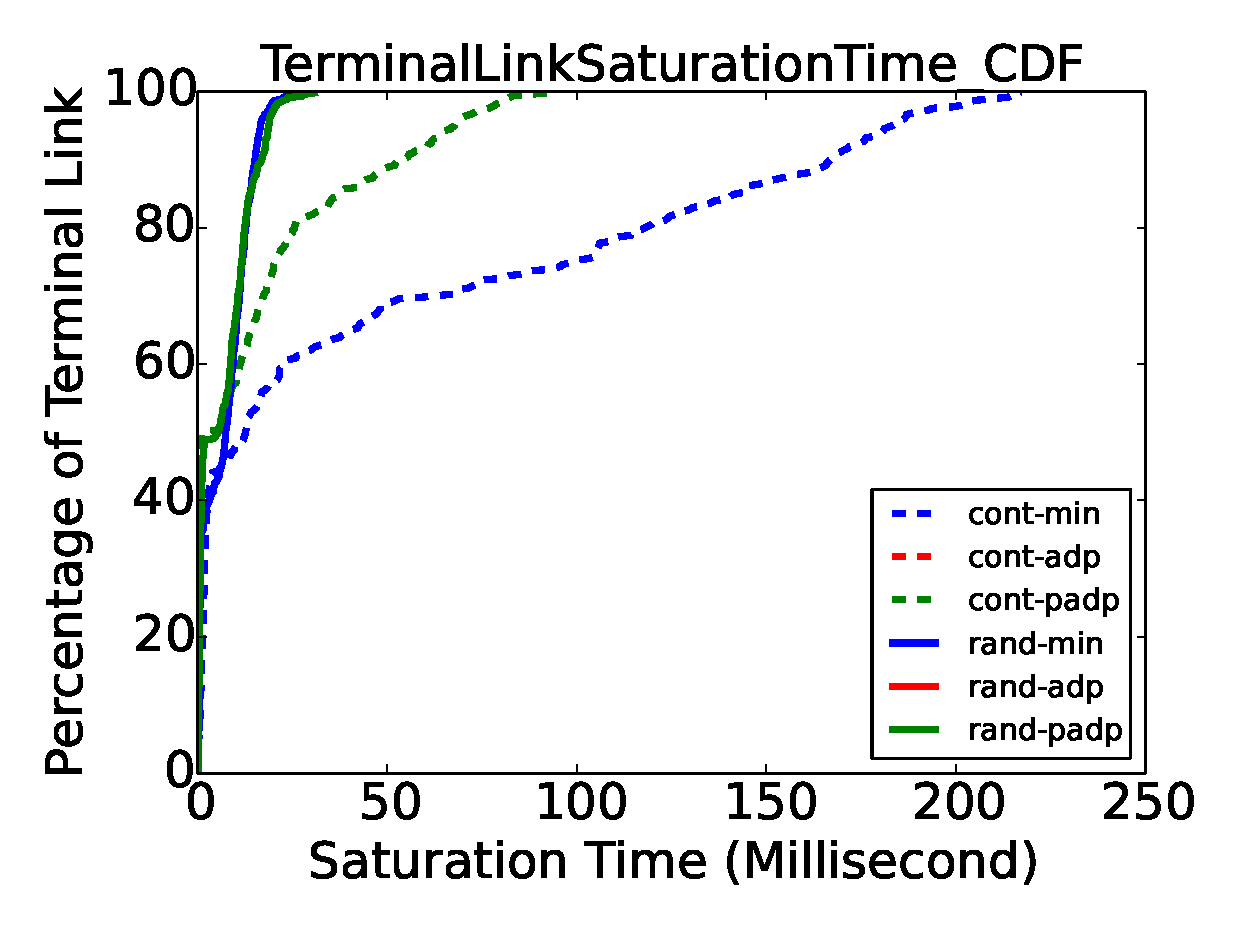
\includegraphics[height=1.8 in]{syn-wkld/tl-btime}
        \caption{Terminal Link Saturated Time}
        \label{fig:synwkld-terminal-link-stime}
    \end{subfigure}%
   \caption{Traffic and Saturated Time of different level of links in the dragonfly network when Workload \Rmnum{2} is running under six different placement and routing configurations.}
   \label{fig:synwkld-network-traffic-stime}
\end{figure*}


%+================================================================
%The average communication time spent by all MPI ranks when Workload~\Rmnum{2} is running under different placement and routing configurations shown in Table~\ref{tab:syn-wkld-commtime}. 
%We can observe the similar pattern as in Table~\ref{tab:wkld-commtime}
%The contiguous placement coupled with minimal routing results in highest communication time. 
%The random placement coupled with minimal routing is the most efficient. 
%Progressive adaptive routing is better than adaptive routing when random placement is in use, 
%and they have comparable results when coupled contiguous placement. 
%Same as Workload~\Rmnum{1}, the network reaches the optimal performance when Workload~\Rmnum{2} is running with random placement and adaptive routing. 
%
%\begin{table}[ht]
%\begin{center}
%\caption{Average time spent on communication by all MPI ranks when Workload II is running on dragonfly network under six different placement and routing configurations.} 
%\label{tab:syn-wkld-commtime}
%%\centering % Centers the table on the page, comment out to left-justify
%\begin{tabular}{l c c c c c c }
%\toprule % Top horizontal line
%\toprule
%&\multicolumn{6}{c}{Placement and Routing Configuration} \\ % Amalgamating several columns into one cell is done using the \multicolumn command as seen on this line
%\cmidrule(l){2-7}
%          & CM & CA & CPA & RM & RA & RPA \\ % Column names row
%\midrule % In-table horizontal line
%Time(ms)  & 3360 & 2204 & 2335 & 1791 & 2367 & 1965 \\ % Content row 1
%
%\midrule % In-table horizontal line
%\bottomrule % Bottom horizontal line
%\end{tabular}
%\end{center}
%\end{table}



\subsection{Individual Application Analysis}
\label{sec: workload-2 app analysis}

We study the performance of each application individually by isolating it from Workload~\Rmnum{2}.   
Figure~\ref{fig:syn-apps-commtime} shows the distribution of communication time of three applications in per rank manner, 
when they running concurrently under six different placement and routing configurations.
The ``bully" in Workload~\Rmnum{1} becomes the ``bullied" in Workload~\Rmnum{2}. 
MultiGrid and CrystalRouter are the less communication-intensive applications in Workload~\Rmnum{2}. 
When random placement coupled with (progressive) adaptive routing is in use, 
MultiGrid and CrystalRouter suffer prolonged communication time, 
as shown in Figure~\ref{fig:syn-mg-commtime}, \ref{fig:syn-cr-commtime}. 
Whereas, sAMG benefits from random placement and (progressive) adaptive routing, 
its communication time drops a lot compared with using contiguous placement, shown in Figure~\ref{fig:syn-samg-commtime}. 
Contiguous placement coupled with minimal routing prevents applications from sharing network resource, 
guaranteeing the performance of less communication-intensive applications like MultiGrid and CrystalRouter 
and causing severe performance degradation to sAMG.

\begin{figure*}[t!]
    \centering
    \begin{subfigure}[t]{0.32\textwidth}
        \centering
        \includegraphics[height=1.5 in]{syn-wkld/mg/commtime}
        \caption{MultiGrid}
        \label{fig:syn-mg-commtime}
    \end{subfigure}%
    \begin{subfigure}[t]{0.32\textwidth}
        \centering
        \includegraphics[height=1.5 in]{syn-wkld/cr/commtime}
        \caption{CrystalRouter}
        \label{fig:syn-cr-commtime}
    \end{subfigure}%
    \hspace{1em}%
    \begin{subfigure}[t]{0.32\textwidth}
        \centering
        \includegraphics[height=1.5 in]{syn-wkld/amg10/commtime}
        \caption{sAMG}
        \label{fig:syn-samg-commtime}
    \end{subfigure}%

   \caption{The communication time of all ranks in each application. Three applications running concurrently on dragonfly network with different placement and routing configurations. The ``bully", sAMG, benefits from random placement and adaptive routing, while the ``bullied", MultiGrid and CrystalRouter, suffer performance degradation.}
   \label{fig:syn-apps-commtime}
\end{figure*}



% explain the network status of sAMG, MG and CR
We look into the network level to scrutinize the traffic through the routers serving each application. 
The routers serving sAMG have high volume of traffic on both local and global channels when contiguous placement is in use, 
shown as the dashed line in Figure~\ref{fig:syn-samg-lc-traffic},~\ref{fig:syn-samg-gc-traffic}.
The random placement can alleviate the local congestion by uniformly distributing the traffic of sAMG over the network, getting more routers involved in serving sAMG, as illustrated by solid lines. 
sAMG benefits from random placement by getting their high volume of traffic being redirected 
from its over-loaded routers to the less busy routers in the network. 
In this case, a majority of those less busy routers are belonging to MultiGrid and CrystalRouter.



%MultiGrid and CrystalRouter are the less communication-intensive applications in Workload~\Rmnum{2}.
When MultiGrid is running with contiguous placement, the serving routers have relatively small volume of traffic on their local and global channels, as shown by the dashed lines in Figure~\ref{fig:syn-mg-lc-traffic},~\ref{fig:syn-mg-gc-traffic}. When coupled with (progressive) adaptive routing, more routers are involved in serving MultiGrid, thus the red and green dashed lines are shorter than the blue one. 
When random placement is in use, the MPI ranks of MultiGrid are randomly distributed across the network and sharing routers with other applications. The routers serving MultiGrid have much more traffic on their local and global channels, as shown by the solid lines in Figure~\ref{fig:syn-mg-lc-traffic},~\ref{fig:syn-mg-gc-traffic}. The increased traffic comes from the ``bully" sAMG. 

CrystalRouter has more data transfer than MultiGrid. However, it still becomes the victim of the ``bully" sAMG. We can observe the similar pattern about CrystalRouter from Figure~\ref{fig:syn-cr-lc-traffic},~\ref{fig:syn-cr-gc-traffic} as MultiGrid. When random placement is in use, the routers serving CrystalRouter have more traffic going through.
The extra traffic comes from from the ``bully" sAMG causing performance degradation to MultiGrid and CrystalRouter. 


\begin{figure*}[t]
    \centering
    \begin{subfigure}[t]{0.32\textwidth}
        \centering
        \includegraphics[height=1.5 in]{syn-wkld/mg/lc-traffic}
        \caption{MultiGrid Local Channel Traffic}
        \label{fig:syn-mg-lc-traffic}
    \end{subfigure}\hfill
    \begin{subfigure}[t]{0.32\textwidth}
        \centering
        \includegraphics[height=1.5 in]{syn-wkld/cr/lc-traffic}
        \caption{CrystalRouter Local Channel Traffic}
        \label{fig:syn-cr-lc-traffic}
    \end{subfigure}\hfill
    \begin{subfigure}[t]{0.32\textwidth}
        \centering
        \includegraphics[height=1.5 in]{syn-wkld/amg10/lc-traffic}
        \caption{sAMG Local Channel Traffic}
        \label{fig:syn-samg-lc-traffic}
    \end{subfigure}\\
    \centering
    \begin{subfigure}[t]{0.32\textwidth}
        \centering
        \includegraphics[height=1.5 in]{syn-wkld/mg/gc-traffic}
        \caption{MultiGrid Global Channel Traffic}
        \label{fig:syn-mg-gc-traffic}
    \end{subfigure}\hfill
    \begin{subfigure}[t]{0.32\textwidth}
        \centering
        \includegraphics[height=1.5 in]{syn-wkld/cr/gc-traffic}
        \caption{CrystalRouter Global Channel Traffic}
        \label{fig:syn-cr-gc-traffic}
    \end{subfigure}\hfill
    \begin{subfigure}[t]{0.32\textwidth}
        \centering
        \includegraphics[height=1.5 in]{syn-wkld/amg10/gc-traffic}
        \caption{sAMG Global Channel Traffic}
        \label{fig:syn-samg-gc-traffic}
    \end{subfigure}
   \caption{The aggregate traffic go through the local and global channels of routers serving specific application. Compared with contiguous placement, More routers are involved in serving each application when random placement is in use.}
   \label{fig:syn-3app-gc-traffic}
\end{figure*}



\subsection{Key Observations}

We have made the following observations from the study with Workload~\Rmnum{2}.

\emph{The application becomes the ``bully" in the workload only because it has more amount of data transfer compared with its concurrently running peers.} The ``bully" takes advantage of the network resource belonging to other applications when network sharing is enabled by random placement and adaptive routing policy. 

\emph{The communication-intensive is a relative metric between concurrently running jobs.} MultiGrid and CrystalRouter are the ``bully" in Workload \Rmnum{1} and they become the ``bullied" when running concurrently with sAMG, since sAMG contributes the dominant portion of traffic in  in Workload \Rmnum{2}.




